%
% File Name     : Protokoll.tex
% Purpose       :
% Creation Date : 02-12-2013
% Last Modified : Mon 09 Dec 2013 01:31:36 PM CET
% Created By    :
%

\documentclass[a4paper,12pt]{article}
\usepackage{amsfonts}
\usepackage{listings}
\usepackage{tabularx}
\usepackage[utf8]{inputenc}
\usepackage[ngerman]{babel}
\usepackage{fancyhdr}
\usepackage{amsmath}
\usepackage{graphicx}
\usepackage[hidelinks]{hyperref}
\usepackage{biblatex}

\pagestyle{fancy}

\fancyhead[R]{\today}
\fancyhead[L]{Datenbanken}


\begin{document}
\title{Labor Datenbanken Gruppe 10}
\author{ Oliver Gebhard \and Dominic Glienke }
\maketitle

\newpage
\tableofcontents
\newpage
\setcounter{tocdepth}{2}


\section{Einleitung}

\begin{figure}[h]
    \centering
    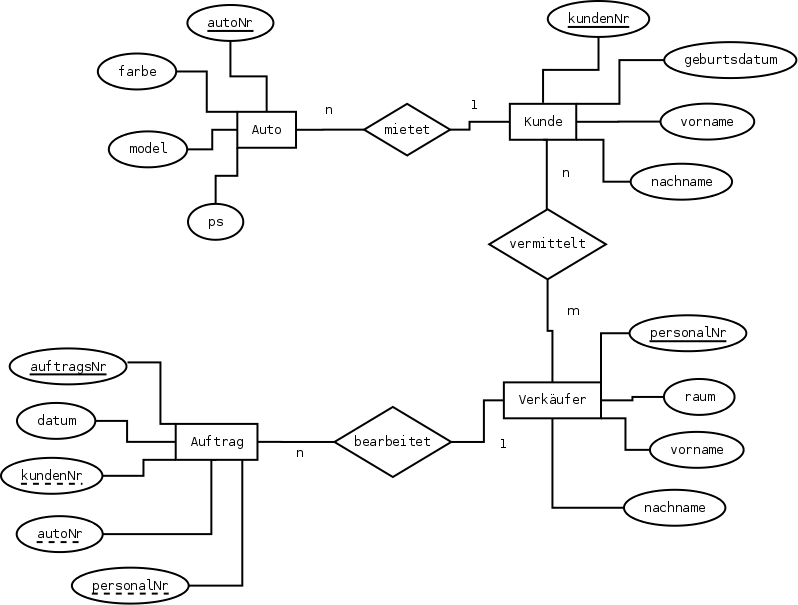
\includegraphics[scale=0.24]{ER_Schema_Autovermietung.png}
    \caption{ER-Schema}
    \label{Autovermietung}
\end{figure}

\newpage

\subsection{Beschreibung}

ER-Schema Autovermietung \\

Folgendes ER-Schema stellt Geschäftsprozesse der Autovermietung im Groben dar. 
Das Entity 	Auto besitzt die Attribute autoNr (Primärchlüssel), farbe, model, ps.
		Kunde besitzt die Attribute kundenNr (Primärschlüssel), geburtsdatum, vorname, nachname.
Mitarbeiter besitzt die Attribute personalNr (Primärschlüssel), raum, vorname, nachname.
Mietet besitzt die Attribute auftragsNr (Primärschlüssel), datum, kundenNr, autoNr, personalNr.

Ein Kunde kann mehrere Autos mieten.  Ein Auto kann mehrfach vermietet werden (n:m).
Ein Auftrag (Mietvorgang) wird von einem Mitarbeiter bearbeitet (1:n).

\newpage
\begin{appendix}
\section{Anhang}

\subsection{SQL}

\lstinputlisting[language=SQL]{statements.sql}

\end{appendix}

\end{document}
